In this Chapter, we define a RL system and its components mathematically as a Markov Decision Process. Then, we introduce some methods to solve a MDP: Exact Solution Methods and Policy Gradient Methods. Finally we present the Advanced Policy Gradient algorithms, which will be used in this work.

\section{Concepts of a Reinforcement Learning System} \label{sec:rlconcepts}

Reinforcement Learning (RL) is learning what to do -- how to map situations to actions -- so as to maximize
a numerical reward signal. The learner is not told which actions to take, but instead must discover
which actions yield the most reward by trying them. In the most interesting and challenging cases,
actions may affect not only the immediate reward but also the next situation and, through that, all
subsequent rewards \cite{sutton1998rli}.

This learning process happens by interacting with the environment where the agent lives and therefore choose its actions. It is basically a ``trial and error" approach as humans or other animals do, but in this case using a computational approach and mathematical modeling.

The origin of modern Reinforcement Learning has two main threads developed outside Artificial Intelligence research. One concerns about trial and error search inside psychology of animal learning, based on Behaviorism theory \cite{skinner1953science} and ``The Law of Effect" \cite{Thorndike173}. The other thread concerns the problem of optimal control and its solution using value functions
and dynamic programming. Both of them contributed for the modern ideas in reinforcement learning, either with the abstractions of learning or mathematical modeling for this problem.

Reinforcement Learning is different from other kinds of Machine Learning, for several reasons:

\begin{itemize}
	\item \textbf{There is no supervisor, only a reward signal}: in Supervised Learning, there is a set of pairs $(x, y)$ and we optimize a cost function in a way to minimize the error from prediction and the ground truth. Therefore, there is a knowledgable external supervisor and a clear specification of mapping between situation and action to take - which doesn't exist in the context of reinforcement.
	
	\item \textbf{Feeback is delayed, not instantaneous}: in Reinforcement Learning, the reward is a consequence of a sequence of actions, rather than a direct mapping from actions to reward. For example, during the learning of a kick motion, the final reward of ball movement only occurs after all the agent motion.
	
	\item \textbf{Data is not independent and identically distributed}: in this kind of learning, there is a intrinsic sequentiality, i.e, the data we collect at some point depends on the state we are.
	
	\item \textbf{Agent's actions affect the subsequent data it receives}: more than being i.i.d data, the learning process itself change the data distribution, differently from supervised learning where the dataset doesn't change during the course of training.
\end{itemize}


Therefore, the optimization problem in Reinforcement Learning has new challenges and needs a different analysis when compared with other kinds of Machine Learning. In this chapter, we will explore these ideas and state-of-art techniques to sustain our experimentations.

\section{Reinforcement Learning System}\label{sec:rlsystem}

Figure \ref{fig:rlsystem} shows how a Reinforcement Learning system works and some of the core concepts involved. As described in section \ref{sec:rlconcepts}, there are two main entities in Reinforcement Learning: an \textit{agent}, which takes actions with the object of accumulate reward, and a \textit{environment}, the place where happens this interaction and whose dynamics affects the decision about these actions.

During learning process, the agents gets a \textit{observation} from the environment and maps to a \textit{state}. Accordingly to that state, the agent then executes an \textit{action} in the environment, based on the current \textit{policy} of actions, which has a consequence in the environment and causes a transition in that state. Furthermore, the agent receives a \textit{reward} signal about how that action affected the environment in terms of accomplish the task goals. This cycle will happen iteratively and the policy will be adjusted in a way that maximize the cumulative reward.

In the next subsections, we will describe in deep the main concepts of a RL system.

\begin{figure}[!htpb]
	\centering
	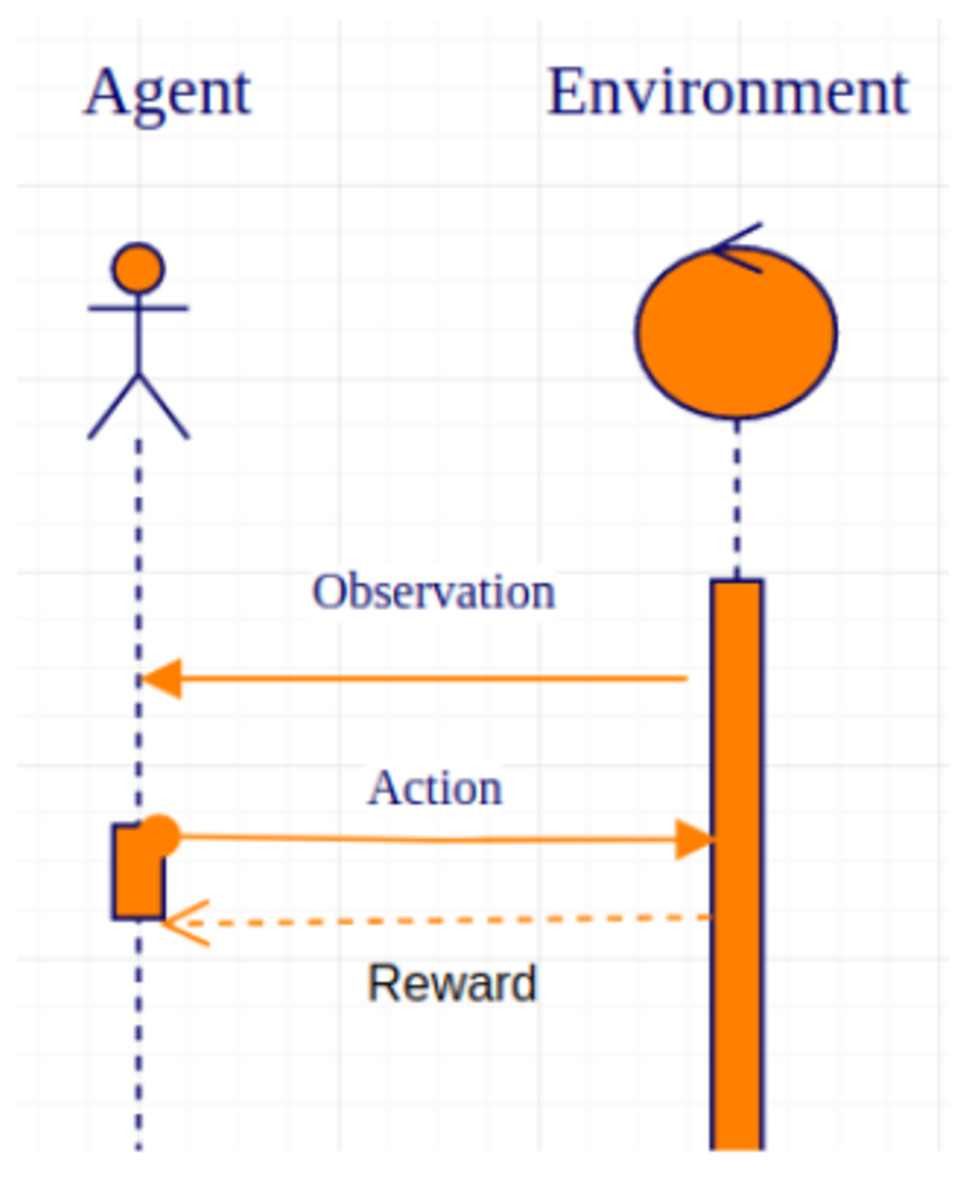
\includegraphics[scale=0.5]{Cap4/rlsystem.eps}
	\caption{Reinforcement Learning System.}
	\label{fig:rlsystem}
\end{figure}

\subsection{Reward}\label{sec:reward}
A reward signal is a scalar number received by the agent and drives the goal in a RL problem. It indicates how well is the action taken in that state. In the learning process, the reward signal guides the policy modification: when an action has high reward, it is a case of positive reinforcement and the policy will be adjusted to take this action more likely in that state; on the other side, if the reward is low, it is a case of negative reinforcement and policy will try to act in this way less times.

Finally, we can formalize this idea stating that RL is based on the \textbf{Reward Hypothesis}:

\begin{definition}
	All goals can be described by the maximization of expected cumulative reward.
\end{definition}

\subsection{State}

Basically, a state is a function of the sequence observations, actions and rewards. There are two different concepts of State:

\begin{itemize}
	\item \textbf{Environment State}: Environment's internal representation - the way it understands its feature at that point and uses to pick next observation or reward.
	\item \textbf{Agent State}: The information that agent perceives and understand from the observation and uses to pick a new action.
\end{itemize}

In RL problems, we commonly use the \textbf{Agent State} concept -- the information provided by the environment and interpreted by the agent in order to decide which action to take next. More specifically, we will use the concept of Markov state, which will be discussed later.

\subsection{Policy}

A policy defines the agent's behavior. It maps states to actions. It corresponds to what in psychology would be called a set of stimulus–response rules or associations \cite{sutton1998rli}. 

The policy is the core element of a RL system. It is sufficient to define the behavior of an agent and therefore is the piece we need after the learning process. There are two kind of policies:

\begin{itemize}
	\item \textbf{Deterministic Policy}, where there is a direct map from state to action. The action taken in each state is always the same:
	
	\begin{equation}\label{eq:detpolicy}
	a = \pi(s).
	\end{equation}
	
	In Equation \ref{eq:detpolicy}, the action $a$ is taken by policy $\pi$ as function of the state $s$.
	
	\item \textbf{Stochastic Policy}, where the map happens from the state to a probability distribution between actions:
	
	\begin{equation}
	\pi (a | s) = \mathbb{P}[A_{t} = a | S_{t} = s].
	\end{equation}
\end{itemize}

\subsection{Value Function}\label{sec:valuefunction}
Whereas the reward signal indicates what is good in an immediate sense, a value function specifies what is good in the long run. The value function is a estimate of reward the agent can expect to accumulate over the future, until a terminal state. 

The value function can be formalized in Equation \ref{eq:valuefunction}:

\begin{equation}\label{eq:valuefunction}
v_{\pi}(s) = \mathbb{E}_{\pi}[R_{t+1} + \gamma R_{t+2} + \gamma^{2} R_{t + 3} + ... | S_{t} = s].
\end{equation}

In Equation \ref{eq:valuefunction}, $v_{\pi}$ represents the value function related to policy $\pi$, as the expectation of cumulative sums of rewards $R$. We also consider a discount factor $\gamma$ which defines how many terms will be considered as infinite sum.

In RL, we focus on choosing actions that bring about states of highest value, not just highest reward. Therefore, it is common to sacrifice immediate rewards to maximize future rewards.

Furthermore, it is much harder to determine value than rewards, because while this is given directly from the environment, that one must be estimated accordingly to data the agent receives. We will describe state-of-art algorithms to predict value function later.

\subsection{Model}

A model is a component that predicts environment's behavior. Basically it will estimate the next state given the agent's action, as formalized in Equation \ref{eq:modelrl}:

\begin{equation}\label{eq:modelrl}
\mathcal{P}_{ss'}^{a} = \mathbb{P}[S_{t+1} = s' | S_{t} = s, A_{t} = a],
\end{equation}
where $\mathcal{P}$ is a transition matrix which calculates the probability of transit between state $s$ and $s'$ given the action $a$.

Models are used for planning, by which we
mean any way of deciding on a course of action by considering possible future situations before they are
actually experienced \cite{sutton1998rli}. There are two methods based on model classification:

\begin{itemize}
	\item \textbf{Model-based RL}, methods that uses model and planning to solve the learning challenge;
	\item \textbf{Model-free RL}, which are methods that are direct trial and error learners.
\end{itemize}

Sometimes there is no model of the environment or it is very hard to create it -- in that cases, we commonly use model-free methods. In this work, we do not know about the dynamics of the Soccer 3D simulator, thus we adopt model-free RL.

\section{Markov Decision Process}

 Markov Decision Processes (MDPs) are a classical
formalization of sequential decision making, where actions influence not just immediate rewards, but also
subsequent situations, or states, and through those future rewards \cite{sutton1998rli}. Thus, MDPs formally describe an environment for Reinforcement Learning. Almost all RL problems can be formalized as MDPs \cite{davidsilverlec2}.

In next subsections, we will define mathematically what is a MDP, its major components and properties.

\subsection{Markov State}\label{sec:markovstate}

A state $S_{t}$ is considered \textit{Markov State} if and only if:

\begin{equation}\label{eq:markovstate}
	\mathbb{P}[S_{t+1} | S_{t}] = \mathbb{P}[S_{t+1} | S_{1},\dots, S_{t}].
\end{equation}

Intuitively, Equation \ref{eq:markovstate} tells that in a Markov State, the future is independent of the past given the present. It means that the state has all the relevant information from the history and therefore it is sufficient statistic for the future. 

As example, consider a chess game: given a specific state -- a set of pieces in the board -- all the information a player needs to play is in the board state, regardless of how the game came in that circumstance. The history may be thrown away.

\subsection{State Transition Matrix}\label{sec:statetransition}

Other major component of a MDP is the State Transition Matrix. Given a set of Markov States, this component defines the probabilities of transition between states. More formally:

\begin{equation}
\mathcal{P} = \begin{bmatrix}
\mathcal{P}_{11} &  \dots  & \mathcal{P}_{1n} \\
\vdots & \ddots & \vdots \\
\mathcal{P}_{n1} &  \dots  & \mathcal{P}_{nn} 
\end{bmatrix},
\end{equation}
where $\mathcal{P}_{ss'}$ is the transition probability:

\begin{equation}
\mathcal{P}_{ss'} = \mathbb{P}[S_{t+1} = s' | S_{t} = s].
\end{equation}

\subsection{Markov Decision Process}

Using the concepts from Subsections \ref{sec:markovstate} and \ref{sec:statetransition}, we can define a \textit{Markov Process} (MP):

\begin{definition}
	A Markov Process, or Markov Chain, is a tuple $(\mathcal{S}, \mathcal{P})$, where:
	\begin{itemize}
		\item $\mathcal{S}$ is a set of states; and
		\item $\mathcal{P}$ is the state transition probability matrix.
	\end{itemize}
\end{definition}

Considering the definition of Markov Process and the concept of Reward described in section \ref{sec:reward}, we can define a \textit{Markov Reward Process} (MRP):

\begin{definition}
	A Markov Reward Process, is a tuple $(\mathcal{S}, \mathcal{P}, \mathcal{R}, \gamma)$, where:
	\begin{itemize}
		\item $\mathcal{S}$ is a set of states; 
		\item $\mathcal{P}$ is the state transition probability matrix;
		\item $\mathcal{R}$ is a reward function, i.e, $\mathcal{R}_{s} = \mathbb{E}[R_{t+1} | S_{t} = s]$; and
		\item $\gamma$ is a discount factor, where $\gamma \in [0,1]$.
	\end{itemize}
\end{definition}

A Markov Reward Process (MRP) describes mathematically an environment in a RL problem. Furthermore, we can differentiate an MRP from a MP by the concept of \textit{Return} that is directly related to the reward over time:

\begin{equation}
G_{t} = R_{t+1} + \gamma R_{t + 2} + \dots = \sum_{k = 0}^{\infty} \gamma^{k} R_{t + k + 1}.
\end{equation}

The idea around cumulative reward was described earlier in section \ref{sec:rlsystem}. However, we need to analyze the discount factor $\gamma$ -- it will weight the trade-off between immediate and delayed rewards. 

Basically, if $\gamma$ is close to zero, the MRP will consider more immediate rewards; on the other side, if $\gamma$ is close to one, the MRP will consider a more delayed reward. Furthermore, the idea of discount is mathematically convenient and avoids infinite returns in cyclic Markov processes \cite{davidsilverlec2}.

Finally, we can extend the idea of MRP by adding an decision making procedure execute by the agent -- which results in the concept of \textit{Markov Decision Process}:

\begin{definition}
		A Markov Decision Process, is a tuple $(\mathcal{S}, \mathcal{A}, \mathcal{P}, \mathcal{R}, \gamma)$, where:
	\begin{itemize}
		\item $\mathcal{S}$ is a set of states; 
		\item $\mathcal{A}$ is a set of actions; 
		\item $\mathcal{P}$ is the state transition probability matrix;
		\item $\mathcal{R}$ is a reward function, i.e, $\mathcal{R}_{s} = \mathbb{E}[R_{t+1} | S_{t} = s]$; and
		\item $\gamma$ is a discount factor, where $\gamma \in [0,1]$.
	\end{itemize}
\end{definition}

Thus, MDP is a MRP with decisions. It worth to mention that the state transition probability $\mathcal{P}$ in MDP also takes in consideration the action executed by the agent:

\begin{equation}
\mathcal{P}_{ss'}^{a} = \mathbb{P}[S_{t+1} = s' | S_{t} = s, A_{t} = a].
\end{equation}

Now, we have a formal definition of a RL problem by using MDP concept. Figure \ref{fig:mdprlsystem} shows the agent-environment interaction in a MDP. In the next section, we will formalize other RL components in a MDP context.

\begin{figure}[ht!]
	\centering
	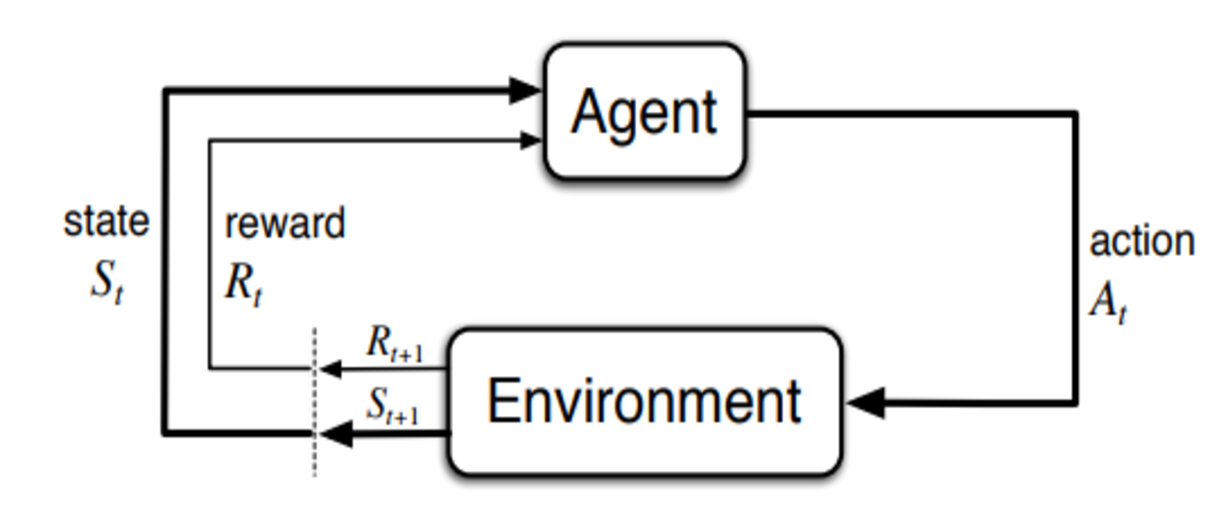
\includegraphics[scale=0.5]{Cap4/mdprlsystem.eps}
	\caption{The agent–environment interaction in a Markov decision process \cite{sutton1998rli}.}
	\label{fig:mdprlsystem}
\end{figure}

\subsection{State-Value and Action-Value Function}

In a MDP context, we can explore deeper the idea of Value Function, and thus define \textit{State-Value} and \textit{Action-Value functions}.

\begin{definition}\label{def:statevalue}
	The state-value function $v_{\pi}(s)$ of a MDP is the expected return starting from $s$ and following a policy $\pi$:
	\begin{equation}
	v_{\pi}(s) = \mathbb{E}_{\pi} [G_{t} \big| S_{t} = s] = \mathbb{E}_{\pi} \left[ \sum_{k = 0}^{\infty} \gamma^{k} R_{t + k + 1} \Bigg| S_{t} = s \right]  ..
	\end{equation}
\end{definition}

The only difference between this definition and the one explained in Section \ref{sec:valuefunction} is the fact that we consider state-value function as a component of a MDP and in terms of return. However, a new concept arises in MDPs: Action-Value function:

\begin{definition}\label{def:actionvalue}
	The action-value function $q_{\pi}(s,a)$ of a MDP is the expected return starting from state $s$, taking action $a$, and then following policy $\pi$ afterwards:
	
	\begin{equation}
	q_{\pi}(s,a) = \mathbb{E}_{\pi} [G_{t} | S_{t} = s, A_{t} = a] = \mathbb{E}_{\pi} \left[ \sum_{k = 0}^{\infty} \gamma^{k} R_{t + k + 1} \Bigg| S_{t} = s, A_{t} = a \right]. 
	\end{equation}
\end{definition}

From definitions \ref{def:statevalue} and \ref{def:actionvalue}, we can see that the action-value function is a granulated version of state-value, considering the new dimension of action space. It is worth to mention that, by definition, the action-value evaluates a specific action in a state, and then follows the policy $\pi$, which means that action $a$ is not chosen by that $\pi$. 

\section{Bellman Equation}

\subsection{Bellman Expectation Equation}

Given definition \ref{def:statevalue}, it is possible to develop state-value function equation and come to a fundamental property of value functions: they satisfy a recursive relationship called \textit{Bellman Equation}:

\begin{align}
v_{\pi} &= \mathbb{E}_{\pi}[G_{t} \mid S_{t} = s] \\
&= \mathbb{E}_{\pi}[R_{t+1} + \gamma R_{t+2} + \gamma^{2} R_{t+3} + \dots \mid S_{t} = s] \\
&= \mathbb{E}_{\pi}[R_{t+1} + \gamma (R_{t+2} + \gamma R_{t+3} + \dots) \mid S_{t} = s] \\
&= \mathbb{E}_{\pi}[R_{t+1} + \gamma v_{\pi}(S_{t+1}) \mid S_{t} = s] \\
&= \sum_{a}\pi(a \mid s) \sum_{s'}\sum_{r} p(s', r \mid s, a) \Bigg[ r + \gamma v_{\pi}(s') \Bigg| S_{t+1} = s'\Bigg].
\label{eq:bellmanbig}
\end{align}

Equation \ref{eq:bellmanbig} can be simplified in terms of reward and transition matrix:

\begin{equation}
v_{\pi}(s) = \mathcal{R}_{s} + \gamma \sum_{s' \in \mathcal{S}}\mathcal{P}_{ss'}v_{\pi}(s').
\label{eq:bellmanfinal}
\end{equation}

The Bellman equation expresses relationship between a state and successor states. Figure \ref{fig:bellmaneqtree} illustrates an agent-environment interaction. This equation average over all the possibilities, weighting by the probability of occurring.

\begin{figure}[!htpb]
	\centering
	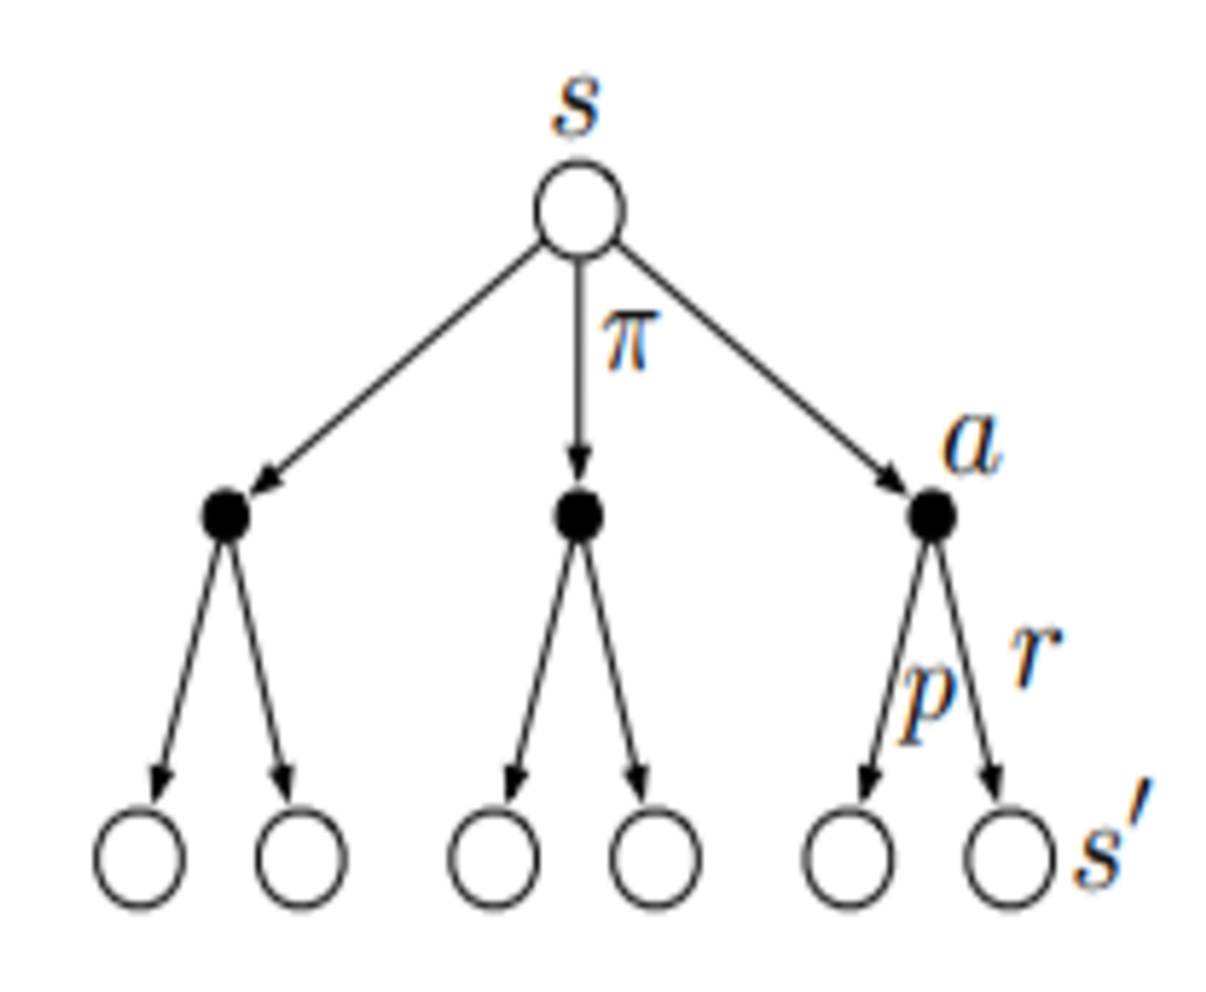
\includegraphics[scale=0.3]{Cap4/bellmaneqtree.eps}
	\caption{Backup diagram for $v_{\pi}$. The white nodes are states, while the black ones are possible actions. Bellman equation average over the actions in a recursive way. \cite{sutton1998rli}.}
	\label{fig:bellmaneqtree}
\end{figure}

The Bellman equation can also be derived for action-value function. Given:

\begin{align}\label{eq:bellmanactionvalue}
q_{\pi}(s,a) = \mathbb{E}_{\pi}[R_{t+1} + \gamma q_{\pi}(S_{t+1}, A_{t+1}) \mid S_{t} = s, A_{t} = a].
\end{align}

It is possible to develop Equation \ref{eq:bellmanactionvalue}, resulting in a version analogous to Equation \eqref{eq:bellmanfinal}:

\begin{equation}
q_{\pi}(s,a) = \mathcal{R}_{s}^{a} + \gamma \sum_{s' \in \mathcal{S}} \mathcal{P}_{ss'}^{a}\sum_{a' \in \mathcal{A}} \pi(a' \mid s')q_{\pi}(s', a').
\end{equation}

The Bellman equation forms the basis of algorithms to learn $v_{\pi}$. The version described here is called \textit{Bellman Expectation Equation} and, as a linear equation, has exact solution. However, there are variations whose purpose is to find optimality in policies and value functions -- and the solution for this methods is not straightforward.

\subsection{Bellman Optimality Equation}

Solving a RL problem means find a policy that its actions results in the maximum cumulative reward. It means find the best policy during learning. We can define optimality for policies based on optimal value functions.

\begin{definition}
	The optimal state-value function $v_{*}(s)$ is the maximum state-value function over all policies:
	\begin{equation}
	v_{*}(s) = \max_{\pi} v_{\pi}(s).
	\end{equation}
	
	Similarly, the optimal action-value function $q_{*}(s,a)$ is the maximum action-value function over all policies:
	\begin{equation}
	q_{*}(s,a) = \max_{\pi} q_{\pi}(s,a).
	\end{equation}
\end{definition}

The optimal value function specifies the best possible performance in the MDP. Therefore, a MDP is considered solved when we know the optimal value function \cite{davidsilverlec2}.

Based on the idea of value function optimality, it is possible to define policy ordering:

\begin{definition}
	Given policies $\pi$, $\pi'$, we can define a partial ordering in the way that
	\begin{align*}
	\forall s \in \mathcal{S}, v_{\pi}(s) \geq v_{\pi'}(s) \Rightarrow \pi \geq \pi'.
	\end{align*}
\end{definition}

Based on this definition, it results in the \textit{Policy Optimality Theorem}:

\newtheorem{optimalpolicy}{Theorem}
\begin{optimalpolicy}
	For any MDP:
	\begin{itemize}
		\item There exists an optimal policy $\pi_{*}$ such that $\pi_{*} \geq \pi, \forall \pi$; and
		\item All optimal policies achieve the optimal state-value and action-value functions: $v_{\pi_{*}}(s) = v_{*}(s)$ and $q_{\pi_{*}}(s,a) = q_{*}(s,a)$.
	\end{itemize}
\end{optimalpolicy}

Also from optimal value function definition, it is possible to define \textit{Bellman Optimality Equation}:

\begin{align}
v_{*}(s) &= \max_{a \in \mathcal{A}(s)} q_{\pi_{*}}(s,a)\\
&= \max_{a} \mathbb{E}[R_{t+1} + \gamma v_{*}(S_{t+1}) \mid S_{t} = s, A_{t} = a]\\
&= \max_{a} \sum_{s', r} p(s', r \mid s, a)[r + \gamma v_{*}(s')]\\
&= \max_{a}\mathcal{R}_{s}^{a} + \gamma \sum_{s' \in \mathcal{S}} \mathcal{P}_{ss'}^{a} v_{*}(s').
\end{align}

Similarly, for action-value function:

\begin{align}
q_{*}(s,a) &= \mathbb{E}[R_{t+1} + \gamma \max_{a'} q_{*} (S_{t+1}, a') \mid S_{t} = s, A_{t} = a] \\
&= \sum_{s',r}p(s',r \mid s,a)[r + \gamma \max_{a'}q_{*}(s',a')] \\
&= \mathcal{R}_{s}^{a} + \gamma \sum_{s' \in \mathcal{S}} \mathcal{P}_{ss'}^{a} \max_{a'} q_{*}(s',a).
\end{align}

Figure \ref{fig:bellmanoptimality} illustrates the Bellman Optimality equation for both state-value and action-value functions, similarly to Figure \ref{fig:bellmaneqtree}. Instead of averaging over actions, the optimality equation chooses the path of greedy action.


\begin{figure}[!htpb]
	\centering
	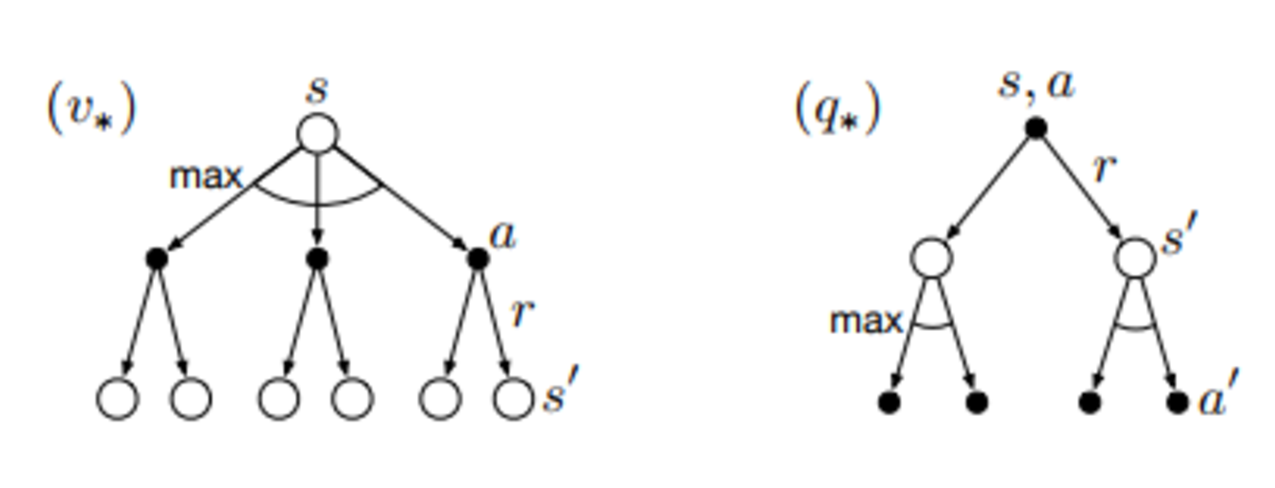
\includegraphics[scale=0.5]{Cap4/bellmanoptimality.eps}
	\caption{Backup diagram in Bellman Optimality Equation for $v_{\pi}$ and $q_{\pi}$. \cite{sutton1998rli}.}
	\label{fig:bellmanoptimality}
\end{figure}

Solving the Bellman Optimality Equation gives the optimal policy for a specific MDP. Therefore, we can conclude that the solution of a RL problem is fundamentally solve this equation. However, as it is non-linear, there is no closed form solution, so we need to explore ways to achieve it.

\section{Exact Solution Methods}\label{sec:exactsolutionmethods}
The first algorithms created to solve the Bellman Optimality Equation in RL problems are based in Dynamic Programming (DP) methods. They require a known MDP model and are, in general, computationally expensive. However, it is important to understand and know their limitations before dive into modern approaches.

The key idea of DP, and of reinforcement learning generally, is the use of value functions to organize
and structure the search for good policies. Thus, the exact solution methods are obtained turning Bellman equations into update rules for improving approximations of the
desired value functions \cite{sutton1998rli}.

\subsection{Policy Iteration}

The first method described here is the Policy Iteration. Figure \ref{fig:policyiteration} illustrates how it works. This technique is composed by two main steps: policy evaluation and policy improvement.


\begin{figure}[!htpb]
	\centering
	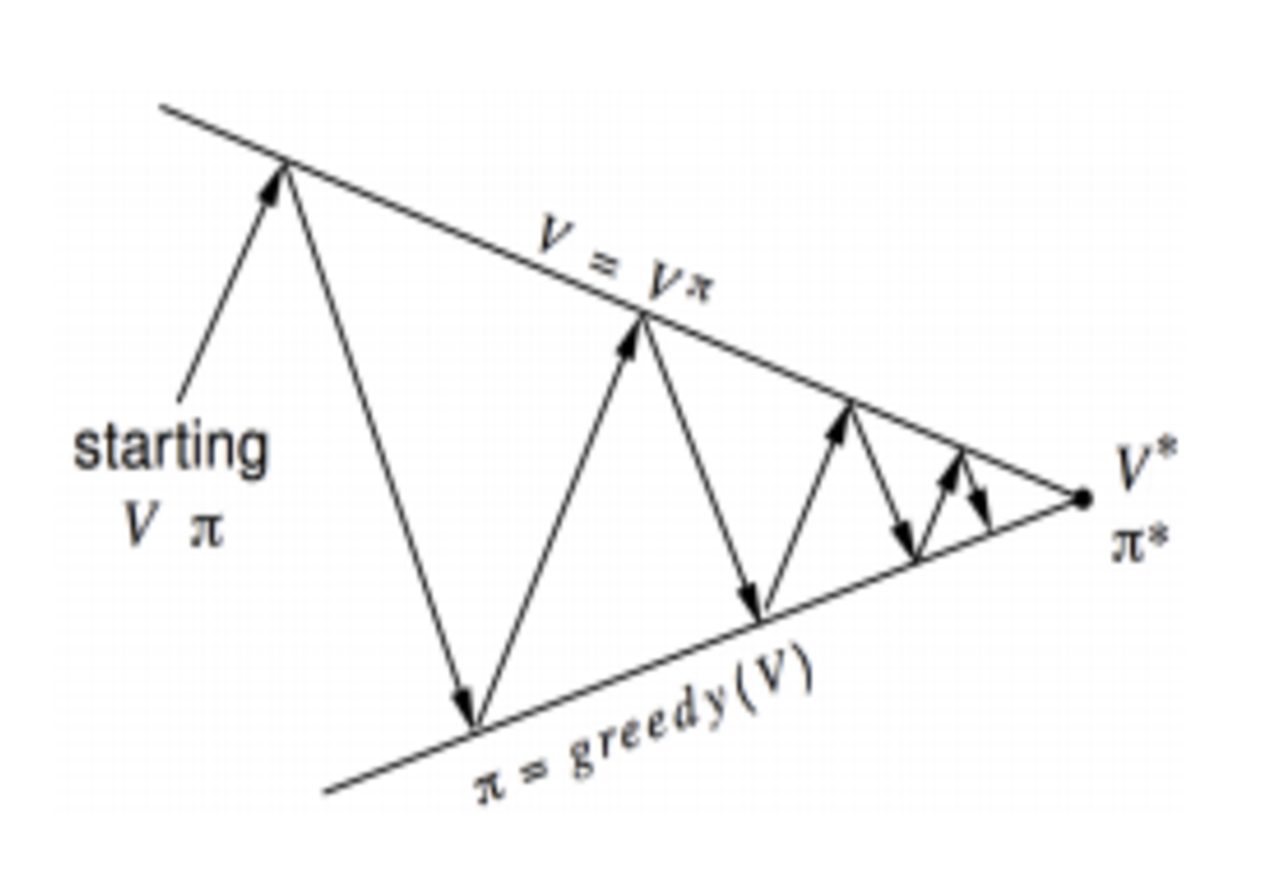
\includegraphics[scale=0.5]{Cap4/policyiteration.eps}
	\caption{Policy Iteration algorithm. \cite{davidsilverlec3}.}
	\label{fig:policyiteration}
\end{figure}

In evaluation, the value function $v_{\pi}$ from the current policy $\pi$ will be estimated. As result, we will have a value function that predicts well the real $v_{\pi}$. Then, it is possible to modify the current policy by taking greedy actions based on the value function, during policy improvement. Basically, we would like to generate $\pi'$ in a way that $\pi' \geq \pi$.

After generating this new policy, we go back to evaluation. This cycle occurs until we find the optimal value function and policy. Therefore, there are two challenges inside policy iteration. We will formulate each of them.

\subsubsection{Policy Evaluation}

During evaluation, we may just apply Bellman updates using the data collected by the agent through the episodes:

\begin{equation}
v_{k+1}(s) = \mathbb{E}_{\pi}[R_{t+1} + \gamma v_{k}(S_{t+1}) \mid S_{t} = s].
\end{equation}

Additionally, it can be shown that:

\begin{equation}
\lim_{k \rightarrow \infty} v_{k} = v_{\pi}.
\end{equation}

Algorithm \ref{alg:policyevaluation} shows the iterative policy evaluation pseudocode.

\begin{algorithm}
	\caption{Iterative Policy Evaluation}
	\begin{algorithmic}
	\REQUIRE $\pi$, current policy
	\REQUIRE $V(s)$, an array for storing value function
	\STATE Initialize $V(s) = 0$ , $\forall s \in \mathcal{S}^{+}$ 
	\STATE \textbf{while} $\delta$ is large enough \textbf{do}
	\STATE \hspace{5mm} $v \leftarrow V(s)$
	\STATE \hspace{5mm} $V(s) \leftarrow \sum_{a} \pi(a \mid s) \sum_{s',r} p(s',r \mid s,a)[r + \gamma V(s')]$
	\STATE \hspace{5mm} $\delta \leftarrow \max(\delta, \lvert v - V(s) \rvert)$
	\STATE \textbf{end while} 	
	\end{algorithmic}
	\label{alg:policyevaluation}	
\end{algorithm}

\subsubsection{Policy Improvement}

During policy improvement, the value function evaluated before will be used to find better policies.

This step is based on \textit{Policy Improvement Theorem}:

\newtheorem{policyimprovement}{Theorem}

\begin{policyimprovement}
	Let $\pi'$ and $\pi$ be any pair of deterministic policies such that, $\forall s \in \mathcal{S}$:
	\begin{equation}
	q_{\pi}(s, \pi'(s)) \geq v_{\pi}(s)
	\end{equation}
	
	Then the policy $\pi'$ must be as good as or better than $\pi$. That is, it must obtain greater or equal expected return from all states $s \in \mathcal{S}$:
	
	\begin{equation}
	v_{\pi'}(s) \geq v_{\pi}(s)
	\end{equation}
\end{policyimprovement}

The proof of this theorem can be found in \cite{sutton1998rli}. Thus, we can improve the policy by acting greedily:

\begin{equation}
\pi'(s) = \argmax_{a \in \mathcal{A}} q_{\pi}(s,a)
\end{equation}

Acting this way, it is possible to satisfy the condition to apply the theorem:

\begin{equation}
q_{\pi}(s,\pi'(s)) = \max_{a \in \mathcal{A}}q_{\pi}(s,a) \geq q_{\pi}(s, \pi(s)) = v_{\pi}(s)
\end{equation}

If the improvement stops, it means the equality has been achieved. Therefore, the Bellman optimality equation has been satisfied:

\begin{equation}
v_{\pi}(s) = \max_{a \in \mathcal{A}} q_{\pi}(s, a) = v_{*}(s)
\end{equation}

\subsubsection{Policy Iteration algorithm}

The policy iteration, as described earlier, is a sequence of evaluations and improvements, until convergence to optimal policy. The Algorithm \ref{alg:policyiteration} shows the pseudocode \cite{sutton1998rli};

\begin{algorithm}
	\caption{Policy Iteration}
	\begin{algorithmic}
		\STATE 1. Initialize $V(s) \in \mathbb{R}$ and $\pi(s) \in \mathcal{A}(s)$ arbitrarily , $\forall s \in \mathcal{S}$ 
		\STATE 2. Run policy evaluation described in Algorithm \ref{alg:policyevaluation}
		\STATE 3. Policy Improvement
		\STATE \hspace{5mm} $policy \_ stable \leftarrow true$
		\STATE \hspace{5mm}\textbf{ For each} $s \in \mathcal{S}$:
		\STATE \hspace{10mm} $old\_action \leftarrow \pi(s)$
		\STATE \hspace{10mm} $\pi(s) \leftarrow \argmax_{a} \sum_{s',r} p(s', r \mid s,a)[r + \gamma V(s')]$
		\STATE \hspace{10mm} \textbf{if} $old\_action \neq \pi(s)$, then $policy \_ stable \leftarrow false$
		\STATE \hspace{5mm} \textbf{if} $policy \_ stable$, then stop and return $V \approx v_{*}$ and $\pi \approx \pi_{*}$; else go to 2.
	\end{algorithmic}
	\label{alg:policyiteration}	
\end{algorithm}

\subsection{Value Iteration}

In the Value Iteration, instead of applying two cyclic steps of evaluation and improvement, the algorithm directly applies Bellman optimality backups. Therefore, this method effectively combines the steps from Policy Iteration, which often results in faster convergence.

Algorithm \ref{alg:valueiteration} presents the pseudocode for this technique.


\begin{algorithm}
	\caption{Value Iteration}
	\begin{algorithmic}

		\STATE Initialize $V(s)$ arbitrarily, $\forall s \in \mathcal{S}^{+}$ 
		\STATE \textbf{while} $\delta$ is large enough \textbf{do}
		\STATE \hspace{5mm} $v \leftarrow V(s)$
		\STATE \hspace{5mm} $V(s) \leftarrow \max_{a} \sum_{s',r} p(s',r \mid s,a)[r + \gamma V(s')]$
		\STATE \hspace{5mm} $\delta \leftarrow \max(\delta, \lvert v - V(s) \rvert)$
		\STATE \textbf{end while} 
		
		\STATE Output a deterministic policy $\pi \approx \pi_{*}$, such that
		\STATE \hspace{5mm} $\pi(s) = \argmax_{a} \sum_{s', r}p(s',r \mid s,a)[r + \gamma V(s')]$	
	\end{algorithmic}
	\label{alg:valueiteration}	
\end{algorithm}

\subsection{Limitations of Exact Solution Methods}

During this section, we presented the core ideas from Exact Solution Methods. They have convergence proofs and are reasonably simple algorithms. However, there are limitation in their uses, which turns inviable in the context of this work.

The first limitation is that these algorithms requires knowledge about the dynamic models. In other words, we need to know about the transition matrix $\mathcal{P}_{ss'}^a$, which turns the usage of these methods very limited. For example, in the case of controlling the kick motion, we need the dynamics of the simulation server and there is not such model.

To solve this problem, many \textbf{sampling-based methods} have been developed. These are model-free RL algorithms and are applied replacing the expectation from Bellman equations by samples of agent executing actions within the environment. From this idea, some methods have arisen, such as \textbf{Monte-Carlo} and \textbf{Temporal-Difference methods}, which resulted in classic algorithms like SARSA \cite{Rummery94on-lineq-learning} and Q-Learning \cite{Watkins:1989}. We will not describe them here for the sake of conciseness. However, the idea of sampling based approximations will be used during experimentation.

The second limitation is about storing and iterating over all states and actions for large MDPs. As described during this Section, using Dynamic Programming requires saving values for each state or action-state. It does not scale well, especially for high dimensional continuous domains like the environment used in this work. For example, in the game of Go, there are $10^{170}$ possible states. If we represent each state with a single bit, we would use approximately $10^{160}$ gigabytes -- there is no capacity in the world for it. Furthermore, there will be a large number of iterations to learn all values individually.

To overcome this problem, the solution is to approximate the value function or even the policy itself using a learning representation:

\begin{align}
\hat v (s, \boldsymbol{\theta} ) \approx v_\pi(s), \\
\hat q (s, a, \boldsymbol{\theta}) \approx q_\pi(q,a). \\
\pi_{\boldsymbol{\theta}}(s,a) \approx \pi(s,a).
\end{align}


The idea behind this is that we can represent all states in a compact way and, during training, generalize from seen to unseen states \cite{davidsilverlec6}. 

We will use neural networks, for some reasons. First, it is differentiable, thus it is possible to use gradient methods for learning. Second, it allows to use data which is not stationary, independent or identically distributed. Lastly, we can use Deep Learning -- shown in Chapter \ref{ch:deeplearning} -- to scale up learning, both in capacity and convergence velocity.

In next sections, we will define policy gradient methods and describe the major algorithms used in this work.


\section{Policy Gradient Methods}\label{sec:pgmethods}

In Policy Gradient Methods, the objective is to learn a parameterized policy that can select actions without consulting a value function, which can be used just for training purposes. These methods compute the gradient for some cost function $J(\theta$) with respect to policy parameters, in a way to maximize the performance.

The usage of policy-based algorithms has some advantages. Firstly, parameterize a policy $\pi$ is often simpler than value functions. Furthermore, $v_{\pi}(s)$ does not prescribe actions (thus would need dynamics modeling and Bellman updates) and $q_{\pi}(s,a)$ need to efficiently solve $\argmax_{a} q_{\pi}(s,a)$, which can be challenging for continuous problems \cite{deeprlbootcamplec4}.

Computing gradients ensures better convergence properties and is effective in continuous action spaces. Additionally, we can learning stochastic policies. The disadvantages are sub-optimality convergence and policy evaluation becomes challenging because is typically inefficient and have high variance \cite{davidsilverlec7}.

Finally, policy direct optimization is useful because it is possible to optimize what we effectively care about and in a compatible way with richer architectures (such as deep neural networks).

\subsection{Policy Gradient Theorem}

There is a excellent theoretical answer which ensures that in parameterized policies, the gradient does not depends on the dynamics model, i.e, it does not involve the derivative of state distribution.

\newtheorem{pg}{Theorem}
\begin{pg}
	Suppose a differentiable parameterized policy that will be optimized using gradient by some performance measure $J(\theta)$. Then:
	
	\begin{equation}
	\nabla J(\boldsymbol{\theta}) \propto \sum_{s}\mu(s)\sum_{a} q_{\pi}(s, a)\nabla_{\boldsymbol{\theta}} \pi(a \mid s, \boldsymbol{\theta}).
	\end{equation}
\end{pg}

Where $\mu$ means the on-policy distribution under $\pi$. The proof for episodic case can be found in \cite{sutton1998rli}. This result is very useful for model-free RL methods.

To apply Policy Gradient Theorem, we need a performance measure $J(\theta)$. In a first moment, let us consider the value function over a episode under policy $\pi$. Let $\tau$ denote a sequence of states and actions in a episode of length $H$ under policy $\pi$. Thus:

\begin{align}
J(\boldsymbol{\theta})  = v_{\pi_{\boldsymbol{\theta}}}(s)
 = \mathbb{E}_{\pi_{\boldsymbol{\theta}}}\Bigg[ \sum_{t = 0}^{H}R_{t}(s, a) \Bigg] = \sum_{\tau} p(\tau, \boldsymbol{\theta}) R(\tau).
\end{align}

For estimating this value, we can use the \textbf{importance sampling method} \cite{NIPS2010_3922} from statistics as ``surrogate loss". This technique works as a variance reduction method where we pick samples from a parameter distribution (denoted here as $\boldsymbol{\theta}_{old}$), but computes the performance measure within respect to a distribution $\theta$ applying a ``importance correction" to the reward:

\begin{equation}\label{eq:optloss1}
J(\boldsymbol{\theta}) = \mathbb{E}_{\tau \sim \boldsymbol{\theta}_{old}} \Bigg[\frac{p(\tau \mid \boldsymbol{\theta})}{p(\tau \mid \boldsymbol{\theta}_{old})}R(\tau) \Bigg].
\end{equation}

Applying the gradient:

\begin{equation}
\nabla_{\boldsymbol{\theta}} J(\boldsymbol{\theta}) = \mathbb{E}_{\tau \sim \boldsymbol{\theta}_{old}} \Bigg[\frac{\nabla_{\boldsymbol{\theta}} p(\tau \mid \boldsymbol{\theta})}{p(\tau \mid \boldsymbol{\theta}_{old})}R(\tau) \Bigg].
\end{equation}

When $\boldsymbol{\theta} = \boldsymbol{\theta}_{old}$:

\begin{align}
\nabla_{\boldsymbol{\theta}} J(\boldsymbol{\theta}) |_{\boldsymbol{\theta} = \boldsymbol{\theta}_{old}} &= \mathbb{E}_{\tau \sim \boldsymbol{\theta}_{old}} \Bigg[\frac{\nabla_{\boldsymbol{\theta}} p(\tau \mid \boldsymbol{\theta})|_{\boldsymbol{\theta} = \boldsymbol{\theta}_{old}}}{p(\tau \mid \boldsymbol{\theta}_{old})}R(\tau) \Bigg] \\
&= \mathbb{E}_{\tau \sim \boldsymbol{\theta}_{old}} [\nabla_{\boldsymbol{\theta}} \log p(\tau \mid \boldsymbol{\theta} ) |_{\boldsymbol{\theta}_{old}}R(\tau)].
\end{align} 

Decomposing this last result in terms of states and actions:

\begin{align}
\mathbb{E}_{\tau \sim \boldsymbol{\theta}_{old}} [\nabla_{\boldsymbol{\theta}} \log p(\tau \mid \boldsymbol{\theta} ) |_{\boldsymbol{\theta}_{old}}R(\tau)] &= \\
&=  \mathbb{E}_{\tau \sim \boldsymbol{\theta}_{old}} \Bigg[\nabla_{\boldsymbol{\theta}} \log \Big[ \prod_{t = 0}^{H}p(s_{t+1}|s_{t}, a_{t})\pi_{\boldsymbol{\theta}}(a_{t}|s_{t})\Big] R(\tau) \Bigg] \\
&= \mathbb{E}_{\tau \sim \boldsymbol{\theta}_{old}} \Bigg[ \nabla_{\boldsymbol{\theta}} \Big[ \sum_{t=0}^{H} \log p(s_{t+1}|s_{t}, a_{t}) + \sum_{t = 0}^{H} \log \pi_{\boldsymbol{\theta}}(a_{t}|s_{t}) \Big] R(\tau) \Bigg] \\
&= \mathbb{E}_{\tau \sim \boldsymbol{\theta}_{old}} \Bigg[ \sum_{t=0}^{H} \nabla_{\boldsymbol{\theta}} \log \pi_{\boldsymbol{\theta}} (a_{t}|s_{t}) R(\tau) \Bigg]. \label{eq:gradnodynamics}
\end{align}

From Equation \eqref{eq:gradnodynamics}, we finally conclude that computing the gradient from the surrogate loss based on importance sampling estimate we have the same result of Policy Gradient Theorem -- which means we have a unbiased estimate of gradient that do not require the dynamics model.

However, even with importance sampling, the gradient estimate is very noisy. We will reduce this variance by using three fixes: using a \textit{Critic}, computing the advantage function instead of value function and changing the surrogate loss to consider KL-divergence trust region. 

\subsection{Actor-Critic Models}

During section \ref{sec:exactsolutionmethods}, we focused on value-based methods, i.e, we chose actions accordingly to value function estimations. On the other side, the current section detailed the usage of Policy Gradient Methods, where we parameterize a policy and apply gradient updates directly. The problem is the high variance, as described in the last subsection.

It is possible to join both ideas in order to reduce variance for Policy Gradient Methods. We use a \textit{Critic} to estimate the action-value function:

\begin{equation}
Q(s, a, \boldsymbol{w}) \approx Q_{\pi_{\boldsymbol{\theta}}}(s,a). 
\end{equation}

Where $\boldsymbol{w}$ represents the parameters of action-value function. Therefore, there are two entities in a Actor-Critic model:

\begin{itemize}
	\item \textbf{Critic} updates action-value function, with parameters $\boldsymbol{w}$;
	\item \textbf{Actor} updates policy parameters $\boldsymbol{\theta}$, in direction suggested by critic
\end{itemize}

In this context, Actor-Critic methods apply a generalization of Policy Iteration algorithm, illustrated by Figure \ref{fig:policyiteration}: while the Critic solves policy evaluation, Actor executes policy improvement.

Furthermore, with the usage of Critic estimating action-value function, Equation \eqref{eq:gradnodynamics} replaces instantaneous for long-term action-value, which also reduces variance:

\begin{equation}
\nabla_{\boldsymbol{\theta}} J(\boldsymbol{\theta}) = \mathbb{E}_{t} \Bigg[ \sum_{t=0}^{H} \nabla_{\boldsymbol{\theta}} \log \pi_{\boldsymbol{\theta}} (a_{t}|s_{t}) Q_{\pi_{\boldsymbol{\theta}}}(s_{t},a_{t}) \Bigg].
\end{equation}


Figure \ref{fig:actorcritic} illustrates how Actor-Critic works.

\begin{figure}[!htpb]
	\centering
	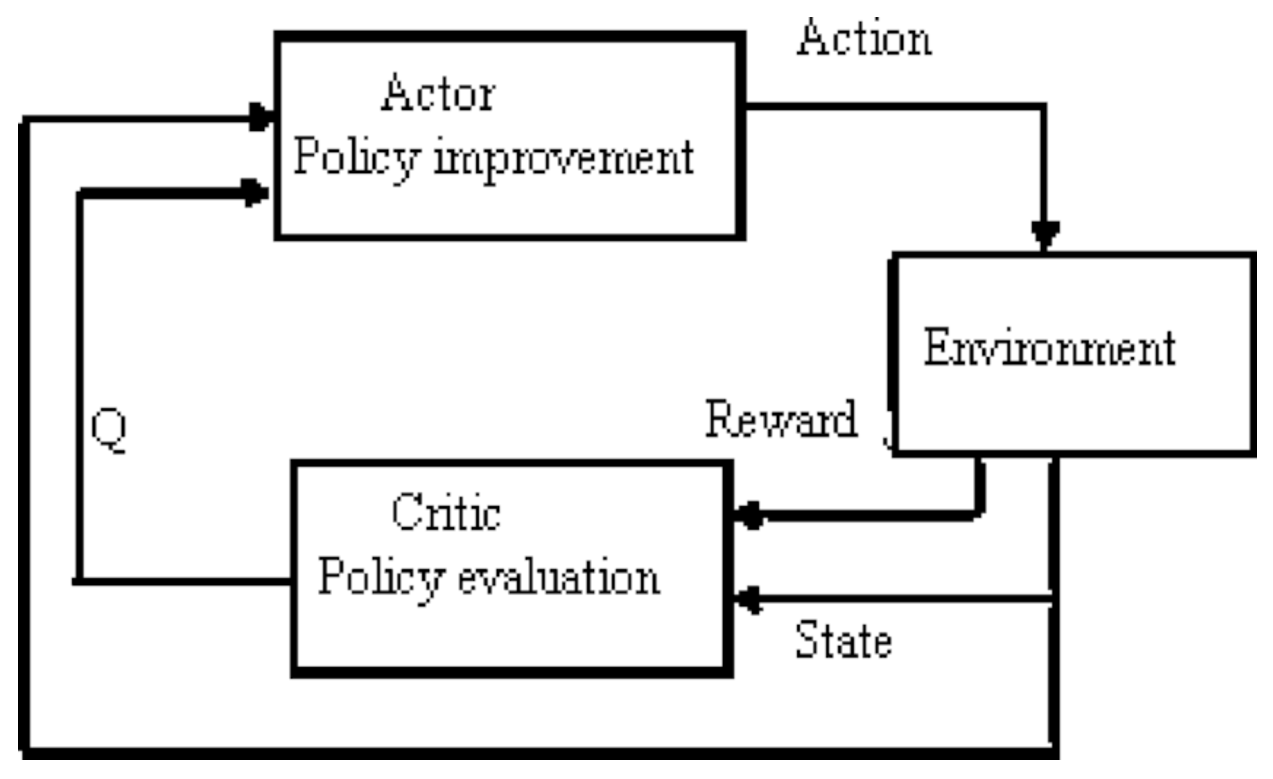
\includegraphics[scale=0.5]{Cap4/actorcritic.eps}
	\caption{Actor-Critic model \cite{actorcritic}.}
	\label{fig:actorcritic}
\end{figure}

\subsection{Advantage Function and GAE Algorithm} \label{sec:gae}

Another idea aiming to reduce variance in Policy Gradient methods is to estimate the Advantage Function instead of action-value. By definition:

\begin{equation}
A_{\pi_{\boldsymbol{\theta}}}(s,a) =Q_{\pi_{\boldsymbol{\theta}}}(s,a) - V_{\pi_{\boldsymbol{\theta}}}(s).
\end{equation}

Using Advantage Function, we estimate both action-value and value-function values. Thus, the performance measure given by Equation \ref{eq:gradnodynamics} changes again:

\begin{equation}\label{eq:advgradient}
\nabla_{\boldsymbol{\theta}} J(\boldsymbol{\theta}) = \mathbb{E}_{t} \Bigg[ \sum_{t=0}^{H} \nabla_{\boldsymbol{\theta}} \log \pi_{\boldsymbol{\theta}} (a_{t}|s_{t}) A_{\pi_{\boldsymbol{\theta}}}(s_{t},a_{t}) \Bigg].
\end{equation}

In practice, in order to estimate Advantage function, it is possible to use Temporal-Difference error:

\begin{equation}
\delta^{t}_{\pi_{\boldsymbol{\theta}}} = R_{s_{t}s_{t+1}} + \gamma V_v(s_{t+1}) - V_v(s_{t}). \label{eq:tderror}
\end{equation}

Where $V_{\boldsymbol{v}}$ is a estimation of $V_{\pi_{\boldsymbol{\theta}}}$, parameterized by $v$. This is possible because Temporal-Difference error estimates Advantage function without bias when $V_{v} = V_{\pi_{\boldsymbol{\theta}}}(s)$ :

\begin{align}
\mathbb{E}_{\pi_{\boldsymbol{\theta}}}[\delta^{t}_{\pi_{\boldsymbol{\theta}}} \mid s_{t},a] 
&= \mathbb{E}_{\pi_{\boldsymbol{\theta}}}[ R_{s_{t}s_{t+1}} + \gamma V_{\pi_{\boldsymbol{\theta}}}(s_{t+1})] - V_{\pi_{\boldsymbol{\theta}}}(s_{t}) \\
&= Q_{\pi_{\boldsymbol{\theta}}}(s_{t},a) - V_{\pi_{\boldsymbol{\theta}}}(s_{t}) \\
&= A_{\pi_{\boldsymbol{\theta}}}(s_{t},a).
\end{align}

However, we cannot guarantee the condition $V_{v} = V_{\pi_{\boldsymbol{\theta}}}(s)$. Thus, this estimation induce bias. To solve this problem, let's define the Advantage Estimator in terms of discounted Temporal-Difference errors of higher orders, e.g:

\begin{align}
A^{(1)}_{\pi_{\boldsymbol{\theta}}, t}(s_{t},a) &= \delta_{\pi_{\boldsymbol{\theta}}, t}. \\
A^{(2)}_{\pi_{\boldsymbol{\theta}}, t}(s_{t},a) &= \delta_{\pi_{\boldsymbol{\theta}}, t} + \gamma \delta_{\pi_{\boldsymbol{\theta}}, t + 1}. \\
A^{(3)}_{\pi_{\boldsymbol{\theta}}, t}(s_{t},a) &= \delta_{\pi_{\boldsymbol{\theta}}, t} + \gamma \delta_{\pi_{\boldsymbol{\theta}}, t + 1} + \gamma^{2}  \delta_{\pi_{\boldsymbol{\theta}}, t + 2}.
\end{align}

The Generalized Advantage Estimator GAE is defined as the exponentially-weighted average of these estimators \cite{DBLP:journals/corr/SchulmanMLJA15}. In mathematical terms:

\begin{align}
A^{GAE(\gamma, \lambda)}_{\pi_{\boldsymbol{\theta}}, t}(s_{t},a) &= (1 - \lambda)(A^{(1)}_{\pi_{\boldsymbol{\theta}}, t}(s_{t},a) + \lambda A^{(2)}_{\pi_{\boldsymbol{\theta}}, t}(s_{t},a) + \lambda^{2} A^{(3)}_{\pi_{\boldsymbol{\theta}}, t}(s_{t},a) + \dots)\label{eq:gae1} \\
&= \sum_{t = 0}^{\infty} (\gamma \lambda)^{t} \delta_{\pi_{\boldsymbol{\theta}}, t+1} \label{eq:gae2}
\end{align}

The steps from Equation \eqref{eq:gae1} to \eqref{eq:gae2} can be found in \cite{DBLP:journals/corr/SchulmanMLJA15}. The $\lambda$ term refers to trace decay parameter, which define how many steps will be considered in estimation. GAE with $\lambda = 0$ is the case of Equation \eqref{eq:tderror} and, as mentioned earlier, can induce bias. On the other side, GAE with $\lambda = 1$ does not induce bias regardless of the accuracy of $V_{v}(s)$, but has high variance. Therefore, GAE with $0 \leq \lambda \leq 1$ makes a compromise between bias and variance, controlled by $\lambda$ \cite{DBLP:journals/corr/SchulmanMLJA15}.

In this work, we use a Advantage Actor-Critic model, where this Advantage function is estimated using GAE. In next section, we finalize Reinforcement Learning Background by adding the last piece in the optimization algorithm to reduce variance: consider KL-divergence trust region.

\section{Advanced Policy Gradient Methods}
There is a third method to reduce variance in parameterized policies: consider it as an optimization problem.

Much of modern ML reduce learning to numerical optimization problem. For example, in supervised learning, the object is to minimize training error \cite{deeprlbootcamplec5}.

So, in this section we will present modern policy gradient techniques that represents learning as a optimization problem that allows small updates in the policy using the data sampled.

\subsection{Optimization Loss}
In Equation \ref{eq:optloss1}, we used importance sampling weighted by model probability distributions and derived the Policy Gradient Theorem result. Then, modified the ``target function" from instantaneous reward to advantage estimation.

However, if we consider Equation \eqref{eq:advgradient} again, we may derive the same gradient from the following loss:

\begin{eqnarray}\label{eq:logprobloss}
\mathcal{L}^{PG}(\boldsymbol{\theta}) = \mathbb{E}_{t}\Big[\log{\pi_{\boldsymbol{\theta}}} (a_{t} \mid s_{t} )A_{\pi_{\boldsymbol{\theta}}}(s,a)\Big],
\end{eqnarray}
and, equivalently, we can differentiate the same gradient from this following loss, where we apply importance sampling to policy distribution:

\begin{eqnarray}\label{eq:surrloss}
\mathcal{L}^{PG}(\boldsymbol{\theta}) = \mathbb{E}_{t}\Big[\frac{\pi_{\boldsymbol{\theta}}(a_{t} \mid s_{t})}{\pi_{\boldsymbol{\theta}_{old}}(a_{t} \mid s_{t})}A_{\pi_{\boldsymbol{\theta}}}(s,a)\Big].
\end{eqnarray}

\citeauthor{trpo} and \citeauthor{Kakade02approximatelyoptimal} analyze the usage of Equation \eqref{eq:surrloss} as surrogate loss and concluded that in practice the results are not much different if compared to Equation \ref{eq:logprobloss}, for small policy changes.

The problem of Equation \eqref{eq:surrloss} is because it leads to destructively large policy updates. Thus, we need a way to ensure these step sizes are small enough so a bad update does not collapse policy.
\subsection{Trust Region Policy Optimization -- TRPO}

From Equation \ref{eq:surrloss}, the first method to avoid large policy updates is to define a trust region update and reduce learning to a optimization problem:

\begin{align}\label{eq:tr}
&  \max_{\boldsymbol{\theta}}  \mathbb{E}_{t}\Big[\frac{\pi_{\boldsymbol{\theta}}(a_{t} \mid s_{t})}{\pi_{\boldsymbol{\theta}_{old}}(a_{t} \mid s_{t})}A_{\pi_{\boldsymbol{\theta}}}(s,a)\Big],\\ &  \text{subject to }  \mathbb{E}_{t}[KL[\pi_{\boldsymbol{\theta}_{old}}, \pi_{\boldsymbol{\theta}}]] \leq \delta \nonumber.
\end{align}

This is a constrained optimization problem. The constrain here is a \textbf{Kullback-Leibler divergence}, which measures how a probability distribution is different from a second. In this case, we ensure the value of this divergence is small. Therefore, the policy change is not big, avoiding steps too far away which could collapse learning.

Finally, based on what have been shown in Section \ref{sec:pgmethods} and this one, we present th TRPO algorithm pseudocode.


\begin{algorithm}[!htbp]
	\caption{TRPO Algorithm}
	\begin{algorithmic}
		\STATE \textbf{while} stopping criteria not met \textbf{do}
		\STATE \hspace{5mm} Run policy $\pi$ for $H$ timesteps
		\STATE \hspace{5mm} Estimate Advantage Function at all timesteps
		\STATE \hspace{5mm} Solve the numerical optimization problem:
		\STATE \hspace{5mm} \begin{align*}
		&  \max_{\boldsymbol{\theta}}  \mathbb{E}_{t}\Big[\frac{\pi_{\boldsymbol{\theta}}(a_{t} \mid s_{t})}{\pi_{\boldsymbol{\theta}_{old}}(a_{t} \mid s_{t})}A_{\pi_{\boldsymbol{\theta}}}(s,a)\Big]\\ &  \text{subject to }  \mathbb{E}_{t}[KL[\pi_{\boldsymbol{\theta}_{old}}, \pi_{\boldsymbol{\theta}}]] \leq \delta \nonumber
		\end{align*} 
		\STATE \textbf{end while}
	\end{algorithmic}
	\label{alg:trpo}
\end{algorithm}

The technique proposed to efficiently approximately solve this optimization problem can be found in \cite{trpo} and is based on conjugate gradient method \cite{Hestenes&Stiefel:1952}.

TRPO is a scalable method with strong theoretical foundations, being able to learn controllers for robotics locomotion from scratch for continuous tasks, using a generic policy search method and general purpose policy representation due to its results in classical benchmarking environments.

However, as a constrained optimization problem, it is difficult to implement a solver method based on conjugate gradients. Additionally, is not compatible with architectures that include noise or parameter sharing.


\subsection{Proximal Policy Optimization -- PPO}

The Proximal Policy Optimization (PPO) algorithm have some of the benefits of TRPO, but it is much simpler to implement, more general, and have better sample
complexity empirically \cite{ppoalgorithm}.


\subsubsection{Clipped Surrogate Loss}

As we saw, the trust region method ensures small policy updates by constraining the problem. However, it is really hard to solve the underlying optimization problem efficiently.

What PPO does is to try to ensure small changes by clipping the surrogate loss, penalizing big steps. Let us define:

\begin{eqnarray}
r_{t}(\boldsymbol{\theta}) = \frac{\pi_{\boldsymbol{\theta}}(a_{t} \mid s_{t})}{\pi_{\boldsymbol{\theta}_{old}}(a_{t} \mid s_{t})}.
\end{eqnarray}

The clipped surrogate loss is defined as:

\begin{equation}\label{eq:clipsurrloss}
\mathcal{L}^{CLIP}(\boldsymbol{\theta}) = \mathbb{E}_{t}\Big[ \min(r_{t}(\boldsymbol{\theta})A_{\pi_{\boldsymbol{\theta}}}, clip(r_{t}(\boldsymbol{\theta}), 1 - \epsilon, 1 + \epsilon)A_{\pi_{\boldsymbol{\theta}}})\Big].
\end{equation}

The Equation \eqref{eq:clipsurrloss} modifies the surrogate objective by clipping the probability ratio, which removes the incentive for moving $r_{t}(\boldsymbol{\theta})$ outside of the
interval $[1 - \epsilon, 1 + \epsilon]$. Finally, it takes the minimum of clipped and unclipped objective, so the
final objective is a lower bound (i.e., a pessimistic bound) on the unclipped objective. With this
scheme, it only ignores the change in probability ratio when it would make the objective improve, and we include it when it makes the objective worse \cite{ppoalgorithm}.

Therefore, PPO tries the same idea of delimiting a small region for updates but treats the problem as an unconstrained optimization -- in a way that is possible to apply stochastic gradient descent again. 

\subsubsection{PPO Algorithm}
Finally, let us join everything described in this chapter to detail the PPO algorithm used in this work. First of all, we use an Actor-Critic model where there are two deep neural networks as parameterized policy and value-function. These neural networks are trained using jointly and using the following loss function:
\begin{equation} \label{eq:finalppoloss}
\mathcal{L}^{CLIP + VF + S}(\boldsymbol{\theta}) = \mathbb{E}_{t}[\mathcal{L}^{CLIP}(\boldsymbol{\theta}) - c_{1} \mathcal{L}^{VF}(\boldsymbol{\theta}) + c_{2}S[\pi_{\boldsymbol{\theta}}](s_{t})].
\end{equation}

$\mathcal{L}^{CLIP}(\boldsymbol{\theta})$ denotes the clipped surrogate loss detailed earlier. The second term,  $\mathcal{L}^{VF}(\boldsymbol{\theta})$ is the squared loss from prediction of value function and its value computed by the samples collected. Thus, this term aims to train the Critic network. The third term, denotes a entropy term to ensure sufficient exploration \cite{a2c}.

In order to estimate the advantage function of $\mathcal{L}^{CLIP}(\boldsymbol{\theta})$ term, we use the GAE algorithm, as explained in Subsection \ref{sec:gae}. We use a truncated version which consider a $T$-length trajectory-segment, i.e, we collect $T$ timesteps from an episode and apply Equation \eqref{eq:gae2} in a finite sum.

Lastly, the algorithm runs as a generalized policy iteration technique: we evaluate the policy by using the data collected and perform improvement applying optimization updates from Equation \eqref{eq:finalppoloss} using the Adam algorithm. Algorithm \ref{alg:ppo} shows the pseudocode.


\begin{algorithm}[H]
	\caption{PPO Algorithm}
	\begin{algorithmic}[!htbp]
		\STATE \textbf{while} stopping criteria not met \textbf{do}
		\STATE \hspace{5mm}\textbf{foreach} agent \textbf{do}
		\STATE \hspace{10mm} Run policy $\pi_{\boldsymbol{\theta}_{old}}$ in environment for $T$ timesteps
		\STATE \hspace{10mm} Estimate Advantage Function at all timesteps using truncated GAE algorithm
		\STATE \hspace{5mm} \textbf{end for}
		\STATE \hspace{5mm}Apply $  \nabla\mathcal{L}^{CLIP + VF + S}(\boldsymbol{\theta})$ to networks using Adam algorithm
		\STATE \hspace{5mm} $\boldsymbol{\theta}_{old} \leftarrow \boldsymbol{\theta}$
		\STATE \textbf{end while}
	\end{algorithmic}
	\label{alg:ppo}
\end{algorithm}